\documentclass{article}
% Change "article" to "report" to get rid of page number on title page
\usepackage{amsmath,amsfonts,amsthm,amssymb}
\usepackage{setspace}
\usepackage{Tabbing}
\usepackage{fancyhdr}
\usepackage{lastpage}
\usepackage{extramarks}
\usepackage{chngpage}
\usepackage{soul,color}
\usepackage{graphicx,float,wrapfig}
\graphicspath{ {images/} }
\usepackage{color}
\usepackage{marvosym}

% In case you need to adjust margins:
\topmargin=-0.45in      %
\evensidemargin=0in     %
\oddsidemargin=0in      %
\textwidth=6.5in        %
\textheight=9.0in       %
\headsep=0.25in         %

% Homework Specific Information
\newcommand{\hmwkTitle}{Int. Analysis Project: 8.4 The Gamma Function}
\newcommand{\hmwkDueDate}{Weekday,\ M\ D,\ Y}
\newcommand{\hmwkClass}{MAT\ \#\#\#}
\newcommand{\hmwkClassTime}{2:30}%
\newcommand{\hmwkClassInstructor}{Professor ___}%
\newcommand{\hmwkAuthorName}{Nicole\ Siegel\ \&\ Ilya\ Kukovitskiy}

% Setup the header and footer
\pagestyle{fancy}                                                       %
\lhead{\hmwkAuthorName}                                                 %
%\chead{\hmwkClass\ - \hmwkTitle}  %
\rhead{\firstxmark}                                                     %
\lfoot{\lastxmark}                                                      %
\cfoot{}                                                                %
\rfoot{Page\ \thepage\ of\ \pageref{LastPage}}                          %
\renewcommand\headrulewidth{0.4pt}                                      %
\renewcommand\footrulewidth{0.4pt}                                      %

% This is used to trace down (pin point) problems
% in latexing a document:
%\tracingall

%%%%%%%%%%%%%%%%%%%%%%%%%%%%%%%%%%%%%%%%%%%%%%%%%%%%%%%%%%%%%
% Some tools
\newcommand{\enterProblemHeader}[1]{\nobreak\extramarks{#1}{#1 continued on next page\ldots}\nobreak%
                                    \nobreak\extramarks{#1 (continued)}{#1 continued on next page\ldots}\nobreak}%
\newcommand{\exitProblemHeader}[1]{\nobreak\extramarks{#1 (continued)}{#1 continued on next page\ldots}\nobreak%
                                   \nobreak\extramarks{#1}{}\nobreak}%

\newlength{\labelLength}
\newcommand{\labelAnswer}[2]
  {\settowidth{\labelLength}{#1}%
   \addtolength{\labelLength}{0.25in}%
   \changetext{}{-\labelLength}{}{}{}%
   \noindent\fbox{\begin{minipage}[c]{\columnwidth}#2\end{minipage}}%
   \marginpar{\fbox{#1}}%

   % We put the blank space above in order to make sure this
   % \marginpar gets correctly placed.
   \changetext{}{+\labelLength}{}{}{}}%

\setcounter{secnumdepth}{0}
\newcommand{\homeworkProblemName}{}%
\newcounter{homeworkProblemCounter}%
\newenvironment{homeworkProblem}[1][Problem \arabic{homeworkProblemCounter}]%
  {\stepcounter{homeworkProblemCounter}%
   \renewcommand{\homeworkProblemName}{#1}%
   \section{\homeworkProblemName}%
   \enterProblemHeader{\homeworkProblemName}}%
  {\exitProblemHeader{\homeworkProblemName}}%

\newcommand{\problemAnswer}[1]
  {\noindent\fbox{\begin{minipage}[c]{\columnwidth}#1\end{minipage}}}%

\newcommand{\problemLAnswer}[1]
  {\labelAnswer{\homeworkProblemName}{#1}}

\newcommand{\homeworkSectionName}{}%
\newlength{\homeworkSectionLabelLength}{}%
\newenvironment{homeworkSection}[1]%
  {% We put this space here to make sure we're not connected to the above.
   % Otherwise the changetext can do funny things to the other margin

   \renewcommand{\homeworkSectionName}{#1}%
   %\settowidth{\homeworkSectionLabelLength}{\homeworkSectionName}%
   %\addtolength{\homeworkSectionLabelLength}{0in}%
   \changetext{}{-\homeworkSectionLabelLength}{}{}{}%
   \subsection{\homeworkSectionName}%
   \enterProblemHeader{\homeworkProblemName\ [\homeworkSectionName]}}%
  {\enterProblemHeader{\homeworkProblemName}%

   % We put the blank space above in order to make sure this margin
   % change doesn't happen too soon (otherwise \sectionAnswer's can
   % get ugly about their \marginpar placement.
   \changetext{}{+\homeworkSectionLabelLength}{}{}{}}%

\newcommand{\sectionAnswer}[1]
  {% We put this space here to make sure we're disconnected from the previous
   % passage

   {\noindent\fbox{\begin{minipage}[c]{\columnwidth}#1\end{minipage}}}%
   \enterProblemHeader{\homeworkProblemName}\exitProblemHeader{\homeworkProblemName}%
       %\marginpar{\fbox{\homeworkSectionName}}%

   % We put the blank space above in order to make sure this
   % \marginpar gets correctly placed.
   }%

%%%%%%%%%%%%%%%%%%%%%%%%%%%%%%%%%%%%%%%%%%%%%%%%%%%%%%%%%%%%%


%%%%%%%%%%%%%%%%%%%%%%%%%%%%%%%%%%%%%%%%%%%%%%%%%%%%%%%%%%%%%
% Make title
\title{\vspace{2in}\textmd{\textbf{\hmwkTitle}}\\\normalsize\vspace{0.1in}\\\vspace{3in}}
\date{}
\author{\textbf{\hmwkAuthorName}}
%%%%%%%%%%%%%%%%%%%%%%%%%%%%%%%%%%%%%%%%%%%%%%%%%%%%%%%%%%%%%

\begin{document}
\begin{spacing}{1.1}
\maketitle

\newpage
% Uncomment the \tableofcontents and \newpage lines to get a Contents page
% Uncomment the \setcounter line as well if you do NOT want subsections
%       listed in Contents
%\setcounter{tocdepth}{1}
\tableofcontents
%\newpage

% When problems are long, it may be desirable to put a \newpage or a
% \clearpage before each homeworkProblem environment

\newpage
\begin{homeworkProblem}[8.4.1]
    For $n\in\mathbb{N}$, let
    \[ n\# = n+(n-1)+(n-2)+\cdots+2+1 .\]
    \begin{homeworkSection}{(a)}
        Without looking ahead, decide if there is a natural way to define $i.$ $0\#$. How about $ii.$ $(-2)\#$? Conjecture a reasonable value for $iii.$ $\frac{7}{2}\#$

        \sectionAnswer{
                $i.$\\
            Redefine $n\#$ as $n\#+0$. Then $0\#=0$.\\
                $ii.$\\
            Since $n\#$ is the sum of all the values from $n$ to $0$, it seems reasonable that the same should apply for the negative numbers. That is,     \[ (-2)\#=(-2)+(-1)+0=-3 \]
                $iii.$\\
            $\frac{7}{2}$ is trickier. I guess one way is to consider $n\#=\frac{n\#}{1}$ and so $\frac{7\#}{2}\#=\frac{7\#}{2}=\frac{7+6+5+4+3+2+1}{2}=\frac{28}{2}=14$
            \[ 1+2+3+4=8=4\#\not=2\#/2=3/2\text{ , soo.. no.} \]
        }
    \end{homeworkSection}

    \begin{homeworkSection}{(b)}
        Now prove $n\#=\frac{1}{2}n(n+1)$ for all $n\in\mathbb{N}$, and revisit part (a).

        \sectionAnswer{
            \underline{Proof by Induction} $1+2+3+\cdots+n=\frac{1}{2}n(n+1)$\\
            Base Case: $n=1$\\
            \[ 1\overset?{=}\frac{1}{2}1(1+1)=\frac{1}{2}2=1 \]
            Inductive Assumption: $1+2+3+\cdots+k=\frac{1}{2}k(k+1)$ for some $k\in\mathbb{N}$\\
            Inductive Step: Show: $1+2+3+\cdots+n+(n+1)=\frac{1}{2}(n+1)((n+1)+1)$\\
            $1+2+3+\cdots+n+(n+1)=\frac{1}{2}n(n+1)+(n+1)$\\
            $=(n+1)(\frac{1}{2}n+1)$\\
            $=\frac{1}{2}(n+1)(n+2)$\\
            $=\frac{1}{2}(n+1)((n+1)+1)$\\
            $\mathcal{QED}$
        }
    \end{homeworkSection}
\end{homeworkProblem}
\newpage

\homeworkProblem[\underline{The Exponential Function}]
    \textbf{The idea of extending the definition of a function defined on $\mathbb{N}$ to all of $\mathbb{R}$ may at first sound like a somewhat whisical enterprise, but it is perfectly analogous to the way we come to understand a function like $2^x$. Similar to $n!,\ 2^n$ for $n\in\mathbb{N}$ is unambiguous and meaningful the minute we understand multiplication, but something like $2^{-\pi}$ is another matter. Because it is instructive, and because we are going to presently need functions of the form $t^x$, let's take a moment to define exponential functions in a rigorous way.}\\
    Typically the way a function like $2^x$ gets defined on $\mathbb{R}$ is through a series of domain expansions. Starting with $2^n$, we first expand the domain to $\mathbb{Z}$ using reciprocals, then to $\mathbb{Q}$ using roots, and finally to $\mathbb{R}$ using continuity.  \textbf{Although we could follow this strategy, we are going to take a different approach that has the advantage of yielding important properties we need more efficiently.}\\
    \textbf{Step one is to properly define the natural exponential function $e^x$. Back in Chapter 6, we assumed $e^x$ was already defined and showed how it could be represented by its Taylor series. Here we flip this process around. The problem on the table is to rigorously construct a proper definition for $e^x$, and the theory of power series gives us a bedrock foundation on which to build.}
\\\\
\noindent
Define
\[ E(x)=\sum^\infty_{n=0}\frac{x^n}{n!}=1+x+\frac{x^2}{2!}+\frac{x^3}{3!}+\cdots \]

\begin{homeworkProblem}[8.4.2]
    Verify $i.$ that the series converges absolutely for all $x\in\mathbb{R}$, $ii.$ that $E(x)$ is differentiable on $\mathbb{R}$, and $iii.$ $E'(x)=E(x).$\\
    \problemAnswer{
            $i.$\\
        A series $\sum f$ converges absolutely if $\sum |f|$ converges.\\
        So show \( \sum^\infty_{n=0}\left|\frac{x^n}{n!}\right| \) converges.\\
        WLOG, assume $m<n$.\\
        Note $\left|\sum^n_{k=0}\left|\frac{x^k}{k!}\right|-\sum^m_{k=0}\left|\frac{x^k}{k!}\right|\right|=\left|\sum^n_{k=m}\left|\frac{x^k}{k!}\right|\right|$\\
        By Cauchy, it remains to be shown that
        \[ \exists\ N\in\mathbb{N}\ \big|\ \forall\ \epilson>0,\ \left|\sum_{k=0}^n-\sum_{k=0}^m\right|<\epsilon\ \forall\ n,m>N. \]
        Let $N>\frac{|x^{m}|+|x^{m+1}|+\cdots+|x^{n}|}{\epsilon}$\\
        Then $N!>N>\frac{|x^{m}|+|x^{m+1}|+\cdots+|x^{n}|}{\epsilon}$\\
        Hence $\epsilon>\frac{|x^{m}|+|x^{m+1}|+\cdots+|x^{n}|}{N!}>\frac{|x^{m}|}{m!}+\frac{|x^{m+1}|}{(m+1)!}+\cdots+\frac{|x^{n}|}{n!}$\\
        $\therefore \epsilon>\frac{|x^{m}|}{m!}+\frac{|x^{m+1}|}{(m+1)!}+\cdots+\frac{|x^{n}|}{n!}$\\
    %}
    %\problemAnswer{
            $ii.$\\
        Consider each additive piece: $\frac{x^n}{n!}$. This is just a polynomial (really a monomial) with a scalar factor. So this is differentiable, with respect to $x$. Note, $f_n'(x)=\frac{x^n}{n!}' = \frac{n\cdot x^{n-1}}{n!}= \frac{x^{n-1}}{\frac{n!}{n}}=\frac{x^{n-1}}{(n-1)}=f_{n-1}$. So:
        \[ E'(x)=\sum^\infty_{n=0}\frac{x^n}{n!}'=\sum^\infty_{n=1}\frac{x^{n-1}}{(n-1)!}=\sum^\infty_{n=0}\frac{x^n}{n!}=E(x) \]
        So by the Term-ny-term Differentiable Theorem, E(x) is differentiable on $\mathbb{R}$, where $E'(x)=E(x)$.\\
        $\mathcal{QED}$
    }
\end{homeworkProblem}

\begin{homeworkProblem}[8.4.3]
    \begin{homeworkSection}{(a)}
        Use the results of Exercise 2.8.7 and the binomial formula to show that $E(x+y)=E(x)E(y)\ \forall\ x,y\ \in\ \mathbb{R}$\\
        \textbf{2.8.7:}\\
        Assume that $\sum^\infty_{i=1}a_i$ converges absolutely to $A$, and $\sum^\infty_{j=1}b_j$ converges absolutely to $B$.\\
        \begin{enumerate}
            \item Show that the iterated sum $\sum^\infty_{i=1}\sum^\infty_{j=1}\left|a_ib_j\right|$ converges so that we may apply \textbf{Theorem 2.8.1:}\\
            \begin{itemize}
                \item Let $\left\{ a_{ij}:\ i,\ j\ \in\ \mathbb{N} \right\}$ be a doubly indexed array of real numbers. (Matrix.) If
                \[ \sum^\infty_{i=1}\sum^\infty_{j=1}a_{ij} \]
                converges, then both $\sum^\infty_{i=1}\sum^\infty_{j=1}a_{ij}$ and $\sum^\infty_{j=1}\sum^\infty_{i=1}a_{ij}$ converge to the same value. Moreover,
                \[ \lim_{n\to\infty}s_{nn}=\sum^\infty_{i=1}\sum^\infty_{j=1}a_{ij}=\sum^\infty_{j=1}\sum^\infty_{i=1}a_{ij} ,\]
                where $s_{nn}=\sum^n_{i=1}\sum^n_{j=1}a_{ij}$.\\
            \end{itemize}
            \item Let $s_{nn}=\sum^\infty_{i=1}\sum^\infty_{j=1}a_ib_j$, and prove that $\lim_{n\to\infty}s_{nn}=AB$. Conclude that 
            \[ \sum^\infty_{i=1}\sum^\infty_{j=1}a_ib_j=\sum^\infty_{j=1}\sum^\infty_{i=1}a_ib_j=2\sum^\infty_{k=2}d_k=AB \]
            where $d_k=a_1b_{k-1}+a_2b_{k-2}+\cdots+a_{k-1}b_1$.
        \end{enumerate}\\\\
        \noindent
        Note, the product of series:
        \[ \left(\sum^\infty_{i=1}a_i\right)\left(\sum^\infty_{j=1}b_j\right)=\sum^\infty_{k=2}d_k \ ,\]
        where $d_k=a_1b_{k-1}+a_2b_{k-2}+\cdots+a_{k-1}b_1$.
        \sectionAnswer{
            Considering $E(x)E(y)$:\\
            By Exercise 2.8.7, keeping in consideration that the first term has index $0$,\\
            Let $d_k=x\frac{y^{k-1}}{(k-1)!}+\frac{x^2}{2!}\frac{y^{k-2}}{(k-2)!}+\cdots+\frac{x^k}{k!}y=\sum_{l=0}^k\frac{x^l}{l!}\frac{y^{k-l}}{(k-l)!}$\\
            Using this double-summation method:
            \[ 
                \sum_{n=0}^\infty\frac{x^n}{n!}\sum_{m=0}^\infty\frac{y^m}{m!}
                =\sum_{k=0}^\infty d_k=\sum_{k=0}^\infty\sum_{l=0}^k\frac{x^l}{l!}\frac{y^{k-l}}{(k-l)!}
            \]\\
            Considering $E(x+Y)$:\\
            Using the binomial formula:
            \[ 
                \sum_{n=0}^\infty\frac{(x+y)^n}{n!}
                =\sum_{n=0}^\infty\left(\frac{1}{n!}\sum_{l=0}^n\binom{n}{l}x^ly^{n-l}\right)
                =\sum_{n=0}^\infty\left(\frac{1}{n!}\sum_{l=0}^n\left(\frac{n!}{l!(n-l)!}\right)x^ly^{n-l}\right)
            \]
            \[
                =\sum_{n=0}^\infty\left(\sum_{l=0}^n\left(\frac{1}{l!(n-l)!}\right)x^ly^{n-l}\right)
                =\sum_{n=0}^\infty \sum_{l=0}^n \frac{x^ly^{n-l}}{l!(n-l)!} 
            \]
            Which is the same as the double sum above.\\
            $\mathcal{QED}$
        }
\end{homeworkSection}
%\newpage
    \begin{homeworkSection}{(b)}
        Show that $i.$ $E(0)=1,\ ii.\  E(-x)=1/E(x),$ and $iii.\ E(x)>0\ \forall\ x\ \in\ \mathbb{R}.$
    \end{homeworkSection}
    \sectionAnswer{
            $i.$
        \[ E(0)=\sum^\infty_n\frac{(0)^n}{n!}=\frac{1}{1}+\sum^\infty_{n=1}\frac{0^n}{n!}=1+\sum^\infty_{n=1}\frac{0}{n!}=1+0=1 \]
            $ii.$\\
        Apply the product of sums thing from above, as last time.\\
        :(\\
            $iii.$\\
        \textbf{Case 1 $x>0$}\\
        The sum of positive terms is positive.\\
        \textbf{Case 2 $x<0$}\\
        Then $E(x)=1/E(-x)$, where $E(-x)$ is positive by case 1 above, and so $1/E(-x)$ is positive.\\
        \textbf{Case 3 $x=0$}\\
        See $i$, $1>0$.\\
        $\mathcal{QED}$
    }
\end{homeworkProblem}
\vspace{0.5cm}
The takeaway here is that the power series $E(x)$ satisfies all the properties we associate with the exponential function, and we can therefore give ourselves permission to go back to the more familiar notation $e^x$ in place of $E(x)$. What happens if we have a momentary relapse and interpret $e^x$ as the real number $e\approx2.71828\ldots$ raised to the power $x$ rather than $E(x)$? Not to worry - the two interpretations coincide, whenever the former is defined in the usual way.
\newpage
\begin{homeworkProblem}[8.4.4]
    Define $e=E(1)$. Show $i.\ E(n)=e^n$ and $ii.\ E(m/n)=(\sqrt[n]{e})^m$ for all $m,n\in\mathbb{Z}$.\\
    \problemAnswer{\\
            $i.$\\
    \underline{Proof by Induction} $E(n+1)=E(n)E(1)$\\
    Base Case: $E(1)=e^1$\\
    Inductive Assumption: $E(n)=e^n$\\
    Inductive Step: $E(n+1)=E(n)E(1)$\\
    $=e^{n}e=e^{n+1}$\\
    Note, for $n>0$, $E(-n)=\frac{1}{E(n)}=\frac{1}{e^n}=e^{-n}$\\
    Note, for $n=0$, $E(0)=1=e^0$\\ 
            $ii.$\\
    \underline{Proof by Induction}
    $E(\frac{m}{n})=\frac{E(m)}{E(n)}$\\
    Base Case: $m=0, E(\frac{0}{n})=(\sqrt[n]{e})^0=1$\\
    Inductive Assumption: $E(\frac{m}{n})=(\sqrt[n]{e})^m$\\
    Inductive Step: $E(\frac{m+1}{n})=(\sqrt[n]{e})^{m+1}$\\
    $E(\frac{m+1}{n})=E(\frac{m}{n}+\frac{1}{n})=(\sqrt[n]{e})^m + (\sqrt[n]{e})=(\sqrt[n]{e})^{m+1}$\\
    $\mathcal{QED}$
    }
\end{homeworkProblem}

\newpage

\begin{homeworkProblem}[8.4.5]
    Show $\lim_{x\to\infty}x^ne^{-x}=0$ for all $n=0,1,2,\ldots$.\\
    To get started notice that when $x\geq0$, all the terms in $E(x)=\sum\cdots$ are positive.
    
    \problemAnswer{
        Show for all $\epsilon>0$, there exists $M\in\mathbb{R}$ such that whenever $x\geq M$, it follows that $|x^ne^{-x}-0|<\epsilon$ for all $n=0,1,2,\ldots$.\\
        hey $x\geq0\Rightarrow \forall\frac{x^n}{n!}$ are positive...\\\\
        
        \underline{Proof by Induction:}\\
        \textbf{Base Case} $n=0$: Show $\forall\ \epsilon>0,\ \exists M\in\mathbb{R^+}\ s.t.\ e^M<\epsilon$
        
        \textbf{Lemma}
            $\forall\ \epsilon>0,\ e^x<e^{x+\epsilon}\ \forall x\in\mathbb{R}^+$. That is, $e^x$ is increasing when $x>0$.\\
                \[ e^x\overset{?}{<}e^{x+\epsilon} \]
                \[ x^n<(x+\epsilon)^n\ \rightarrow\ e^x=E(x)=\sum_{n=0}^\infty \frac{x^n}{n!}
                <e^{x+\epsilon}=E(x+\epsilon)=\sum_{n-0}^\infty \frac{(x+\epsilon)^n}{n!}
                \]
        Lemma $\mathcal{QED}$
        
        So $\forall\ \epsilon>0,\ \exists M\in\mathbb{R^+}\ s.t.\ e^M<\epsilon$, since $e^{M^+}$ is an increasing unbounded function.
        
        \textbf{Inductive Hypothesis:} Assume $\forall\ \epsilon>0,\ \exists M\in\mathbb{R^+}\ s.t.\ M^n e^M<\epsilon$\\
        \textbf{Inductive Step:} It remains to be shown $\forall\ \epsilon>0,\ \exists M\in\mathbb{R^+}\ s.t.\ M^{n+1} e^{M}<\epsilon$\\
        \[ 
        M^{n+1} e^{M}
        = M(M^n e^{M})
        < \epsilon_1 M_n
        ,\]
        Where $M_n$ is as the hypothesis assumption gives, and $\epsilon_1$ is any positive real number. Let $\epilson_1=\frac{\epsilon}{M_n}$. Then"
        \[ \epsilon_1 M_n = \epsilon .\]
        So
        \[ M^{n+1} e^{M} < \epsilon \]
        $\mathcal{QED}$
    }
\end{homeworkProblem}
\newpage
\noindent
\textbf{Having set $e^x$ on solid mathematical footing}, we can now do the same for $t^x$ where $t>0$. This requires use of the natural logarithm.
\begin{homeworkProblem}[8.4.6]

    \begin{homeworkSection}{(a)}
        Explain why we know $e^x$ has an inverse function - let's call it $\log x$ - defined on the scrictly positive real numbers and satisfying:\\
        \begin{enumerate}
            \item $\log(e^y) = y$ for all $y\in\mathbb{R}$\\
            \item $e^{\log x}=x$ for all $x>0$
        \end{enumerate}
        \sectionAnswer{
            See the beginning of Exercise 5.2.12, below.\\
            Note, $e^x=E(x)=\sum_{n=0}^\infty \frac{x^n}{n!}$ is one-to-one. Then there exists an inverse function defined on the range of $e^x$, that is, defined on $(0,\infty)$.\\
            Calling this function $\log(x):(0,\infty)\to\mathbb{R}$; seeing as it's the inverse of $e^x$, $log(e^y)=y\ \forall y\in\mathbb{R}$ (since $e^y$ is already the domain of this $\log$ function for all real $y$)  and $e^{\log(x)}=x\ \forall x>0$ (since $\log(x)$ must have a positive input to have any meaning).
        }
    \end{homeworkSection}

    \begin{homeworkSection}{(b)}
        Prove $(\log x)'=1/x$. (See exercise 5.2.12.):\\
        \begin{itemize}
            \item If $f:[a,b]\to\mathbb{R}$ is one-to-one, then there exists and inverse function $f^{-1}$ defined on the range of $f$ given by $f^{-1}(y)=x$ where $y=f(x)$. In Exercise 4.5.8 we saw that if $f$ is continuous on $[a,b]$, then $f^{-1}$ is continuous on its domain. Let's add the assumption that $f$ is differentiable on $[a,b]$ with $f'(x)\neq0$ for all $x\in[a,b]$. Show $f^{-1}$ is differentiable with
            \[ (f^{-1})'(y)=\frac{1}{f'(x)} \text{ where } y=f(x) .\]
        \end{itemize}
        \sectionAnswer{
            Note, $e^x$ fits all the assumptions above, it's one-to-one, continuous, and differentiable, and $e'(x)\neq0$. So \( \log(e^x)=\frac{1}{e^x} .\)
            \[ \log(x)=\log(e^{\log x}) = \frac{1}{e^{\log x}} = \frac{1}{x} \]
            $\mathcal{QED}$
        }
    \end{homeworkSection}

    \newpage
    \begin{homeworkSection}{(c)}
        Fix $y>0$ and differentiate $\log(xy)$ with respect to $x$. Conclude that
        \[ \log(xy)=\log x+\log y\text{  for all }x,y>0 .\]
        \sectionAnswer{
            Consider the derivative of $log(xy)'$.
            \[ \frac{d}{dx}\log(xy)=\frac{du}{dx}\frac{d}{du}\log(u) ,\]
            where $u=3x$; and so $du=3dx$, implying $\dfrac{du}{dx}=3$. Note, $\frac{d}{du}log(u)=\frac{1}{u}$. 
            \[ \frac{d}{dx}log(xy)=3\cdot\frac{1}{3x}=\frac{1}{x} \]
            Now, consider the derivative of $log(x)+log(y)$:
            \[ [\log(x)+\log(y)]'_x=[\log(x)]'_x+[\log(y)]'_x=\frac{1}{x}+0=\frac{1}{x} \]
            \[ \begin{array}{lc}
                \log(xy)\bigg|_{x=1} &=\log(y)  \\
                \log(x)+\log(y)\bigg|_{x=1} &=\log(1)+\log(y)=\log(e^0)+\log(y)=0+\log(y)=\log(y) 
            \end{array} \]
            Since $[\log(xy)]'=[\log(x)+\log(y)]'$, and $\log(xy)=log(x)+\log(y)$ for some value $x_0$, $\log(xy)=\log(x)+\log(y)$.
            $\mathcal{QED}$
        }
    \end{homeworkSection}

    \begin{homeworkSection}{(d)}
        For $t>0$ and $n\in\mathbb{N},t^n$ has the usual interpretation as $t\cdot t\cdots t\text{ ($n$ times)}$. Show that
        \[ t^n=e^{n\log t}\text{  for all }n\in\mathbb{N} .\]
        
        \sectionAnswer{
            \[ e^{n\log t}=e^{\log t\cdot \log t\cdots \log t\text{, $n$ times}}=e^{\log t^n}=t^n \]
            $\mathcal{QED}$
        }
    \end{homeworkSection}
    
    \noindent
    \textbf{Part (d) of the previous exercise is the pivotal formula because the expression on the right is meaningful if we replace $n$ with $x\in\mathbb{R}$. This is our cue to use the identity in (2) as a template for the definition of $t^x$ on all of $\mathbb{R}$.
    }

\end{homeworkProblem}

\newpage

\begin{homeworkProblem}[Definition 8.4.2.]
    Given $t>0$, define the exponential function $t^x$ to be 
    \[ t^x=e^{x\log t}\text{ for all } x\in\mathbb{R} \]
\end{homeworkProblem}

\begin{homeworkProblem}[8.4.7]

    \begin{homeworkSection}{(a)}
        Show $t^{m/n}=(\sqrt[n]{t})^m$ for all $m,n\in\mathbb{N}$.
        
        \sectionAnswer{
        Recall $E(m/n)=e^{m/n}=(\sqrt[n]{e})^m$, from Exercise 8.4.4.
            \[ t^{m/n}=e^{(m/n)\log t} = (\sqrt[n]{e}^{m})^{\log t} = \sqrt[n]{e^{\log t}}^m = \sqrt[n]{t}^m \]
            $\mathcal{QED}$
        }
    \end{homeworkSection}

    \begin{homeworkSection}{(b)}
        Show $\log(t^x)=x\log t$, for all $t>0$ and $x\in\mathbb{R}$.
        
        \sectionAnswer{
            Recall $\log(e^y) = y\ \forall y\in\mathbb{R}$, by the definition of $\log(x)$ as the inverse of $e^x$.
            \[ \log(t^x) = \log(e^{x\log t}) = x \log(t) \]
            $\mathcal{QED}$
        }
    \end{homeworkSection}

    \begin{homeworkSection}{(c)}
        Show $t^x$ is differentiable on $\mathbb{R}$ and find the derivative.
        
        \sectionAnswer{
            The derivative that matched was w.r.t. $t$.\\
            Doing w.r.t. $x$, i got $\log t\cdot t^x$.\\
            Recall the Chain Rule, $h(g(x))' = g'(x)\cdot h'(g(x))$.
            \[ \left[ e^{x\log t} \right]'_t = \left[ x\log t \right]'_t\cdot e'^{(x\log t)} = x\frac{1}{t}e^{x\log t} = xt^{x-1} \]
            $\mathcal{QED}$
        }
    \end{homeworkSection}

\end{homeworkProblem}

\newpage

\textbf{
    Finding the right definition for $x!$ is harder than defining $t^x$, but the strategy is essentially the same. We are seeking a formula of the form $n!=g(n)$ where $g$ yields a meaningful formula when $n$ is replaced by $x$. What might such a function $g(x)=x!$ look like when graphed over $\mathbb{R}$? For $x\geq0$ it must grow extremely rapidly to keep up with $n!$, but how about on $x<0$? Using a functional equation for $x!$ we can create a reasonable artist's rendering of the function we are looking for.
}

\homeworkProblem[\underline{The Functional Equation}]
    A defining property of the factorial on $\mathbb{N}$ is that $1!=1$ and $n!=n(n-1)!$ for all $n\geq2$. Thus it seems reasonable to require the same from our currently mythic function $x!$ defined $\mathbb{R}$. Whatever $x!$ means, it should satisfy
    \[ x!=x(x-1)! \text{ for all } x\in\mathbb{R} \]
    Setting $n=1$ in this equation, for example, yields $1=0!$.


\begin{homeworkProblem}[8.4.8]
    Inspired by the fact that $0!=1$ and $1!=1$, let $h(x)$ satisfy
    \begin{enumerate}
        \item $h(x)=1$ for all $0\leq x\leq 1$, and 
        \item $h(x)=xh(x-1)$ for all $x\in\mathbb{R}$.
    \end{enumerate}
    \begin{homeworkSection}{(a)}
        Find a formula for $h(x)$ on $[1,2],\ [2,3],$ and $[n,n+1]$ for arbitrary $n\in\mathbb{N}$.
        \sectionAnswer{
            $h(1)=1$, $h(2)=2\cdot h(1)=2\cdot1=2$
            \[h(x_1), x_1\in(1,2) = x\cdot h(x_1-1)=x_1\cdot 1=x_1\]
            Note, $h(1)=1, h(2)=2$, so this formula for $h(x_1)$ can extend to the domain $x_1\in[1,2]$\\
            $h(2)=2$, $h(3)=3\cdot h(2)=3\cdot 2=6$
            \[h(x_2), x_2\in(2,3) = x\cdot h(x_2-1)=x_2\cdot (x_2-1)\cdot h(x_2-2)=x_2\cdot (x_2-1)\cdot 1=x_2\cdot (x_2-1)\]
            Note, $h(2)=2\cdot 1, h(3)=6=3\cdot 2$, so this formula for $h(x_2)$ can extend to the domain $x_2\in[2,3]$
            \begin{center}
                \begin{multiline} 
                    h(x_n), x_n\in[n,n-1]
                    =x_n\cdot h(x_n-1)
                    =x_n\cdot (x_n-1)\cdot h(x_n-2)\\
                    =x_n\cdot (x_n-1)\cdot (x_n-2)\cdot h(x_n-3)\\
                    =x_n\cdot (x_n-1)\cdot (x_n-2)\cdot\; \cdots\; \cdot (x_n-n-1) \cdot h(x_n-n)\\
                    =x_n\cdot (x_n-1)\cdot (x_n-2)\cdot\; \cdots\; \cdot (x_n-n-1) \cdot 1\\
                    =x_n\cdot (x_n-1)\cdot (x_n-2)\cdot\; \cdots\; \cdot (x_n-n-1)
                \end{multiline}
            \end{center}
        }
    \end{homeworkSection}

    \newpage

    \begin{homeworkSection}{(b)}
        Now do the same for $[-1,0],\ [-2,-1],$ and $[-n,-n+1]$.
        \sectionAnswer{
            Considering $h(x_{-1}), x_{-1}\in(-1,0)$\\
            \[ h(x_{-1}+1)=(x_{-1}+1)h(x_{-1}) \]
            \[ h(x_0)=x_0h(x_{-1}) \]
            \[ \frac{1}{(x_0)}=h(x_{-1}) \]
            \[ \frac{1}{(x_{-1}+1)}=h(x_{-1}) \]
            
            Considering $h(x_{-2}), x_{-2}\in(-2,-1)$\\
            \[ h(x_{-2}+1)=(x_{-2}+1)h(x_{-2}) \]
            \[ h(x_{-1})=x_{-1}h(x_{-2}) \]
            \[ \frac{1}{(x_{-1})(x_{-1}+1)}=h(x_{-2}) \]
            \[ \frac{1}{(x_{-2}+1)(x_{-2}+2)}=h(x_{-2}) \]\\
            Generally:
            \[ h(x_{-n}),x_{-n}\in(-n,-n+1)=\frac{h(x_{-n}+1)}{x_{-n}+1} \]
            \[ =\frac{h(x_{-n}+2)}{(x_{-n}+1)(x_{-n}+2)} \]
            \[ \vdots \]
            \[ =\frac{h(x_-1)}{(x_{-n}+1)(x_{-n}+2)(x_{-n}+(n-1))} \]
            \[ =\frac{1}{(x_{-n}+1)(x_{-n}+2)(x_{-n}+(n-1))(x_{-n}+n)} \]\\
            Considering $h(-1)$:
            \[ \lim_{x_{-1}\to{-1^+}} h(x_1) = \lim\frac{1}{x_{-1}+1}\to\infty \]
            \[ \lim_{x_{-2}\to{-1^-}} h(x_2) = \lim\frac{1}{(x_{-2}+1)(x_{-2}+2)}\to-\infty \]
            \[ \therefore h(-1) DNE \text{, since it's limits from each side are opposite vertical asymptotes.} \]
            Considering $h(-1)$:
            \[ \lim_{x_{-2}\to{-2^+}} h(x_2) = \lim\frac{1}{(x_{-2}+1)(x_{-2}+2)}\to-\infty \]
            \[ \lim_{x_{-3}\to{-2^-}} h(x_3) = \lim\frac{1}{(x_{-3}+1)(x_{-3}+2)(x_{-3}+3)}\to\infty \]
            \[ \therefore h(-2) DNE \text{, since it's limits from each side are opposite vertical asymptotes.} \]
        }
        \sectionAnswer{
            Generally:
            \[ \lim_{x_{-n}\to{-n^+}} h(x_{-n}) = \lim\frac{1}{(x_{-n}+1)(x_{-n}+2)\cdots(x_{-n}+(n-1))(x_{-n}+n)}=\frac{1}{(-)(-)\cdots(-)(x_{-n}+n)}\]
            Note, there are $n-1$ negative factors in the denominator, and $(x_{-n}+n)$ is positive since the limit is approaching from the right. Therefore:
            \[ \lim_{x_{-n}\to{-n^+}} h(x_{-n})
            \left\{
                \begin{array}{ll}
                    \to -\infty & n\text{ even} \\
                    \to \infty & n\text{ odd}
                \end{array}
            \right.
            \]
            \[ \lim_{x_{-n-1}\to{-n^-}} h(x_{-n-1}) = \lim\frac{1}{(x_{-n-1}+1)(x_{-n-1}+2)\cdots(x_{-n-1}+(n))(x_{-n-1}+(n+1)}\]
            \[=\frac{1}{(-)(-)\cdots(-)(x_{-n}+n)(x_{-n-1}+(n+1))} \]
            Note, there are $n-1$ negative factors in the denominator, $x_{-n-1}+n$ is negative since the limit is approaching from the left, and $x_{-n-1}+n+1\approx1$. Therefore:
            \[ \lim_{x_{-n-1}\to{-n^-}} h(x_{-n-1})
            \left\{
                \begin{array}{ll}
                    \to \infty & n\text{ even} \\
                    \to -\infty & n\text{ odd}
                \end{array}
            \right.
            \]
            $\mathcal{QED}$
        }
    \end{homeworkSection}

    \begin{homeworkSection}{(c)}
        Sketch $h$ over the domain $[-4,4]$.
        \sectionAnswer{
            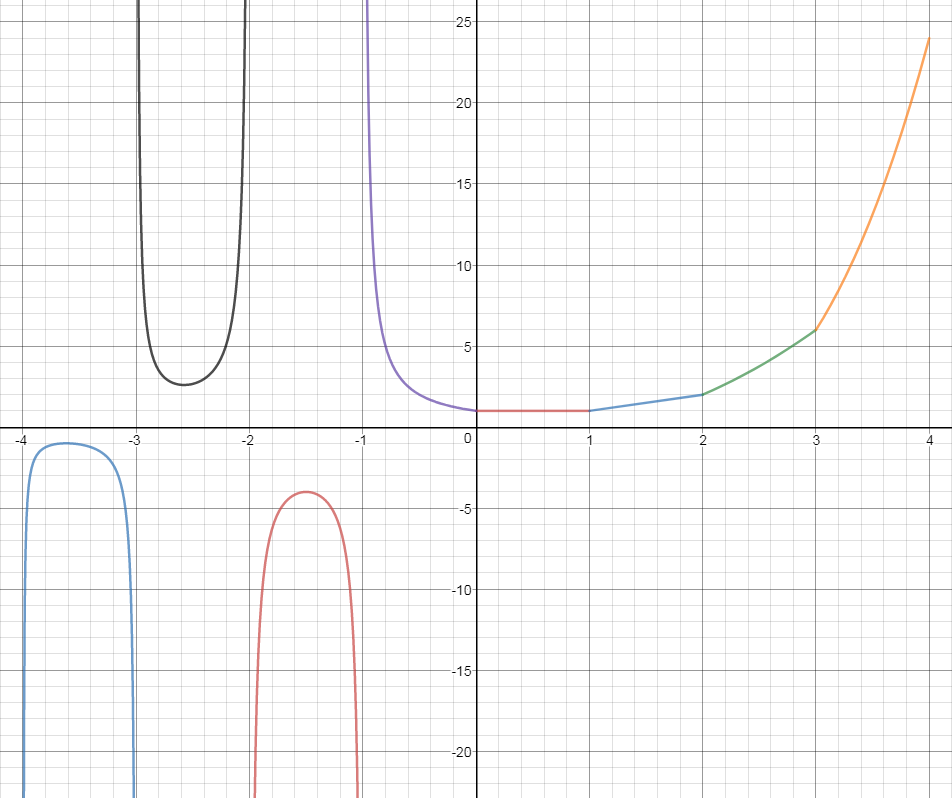
\includegraphics[scale=0.4]{Graph}
            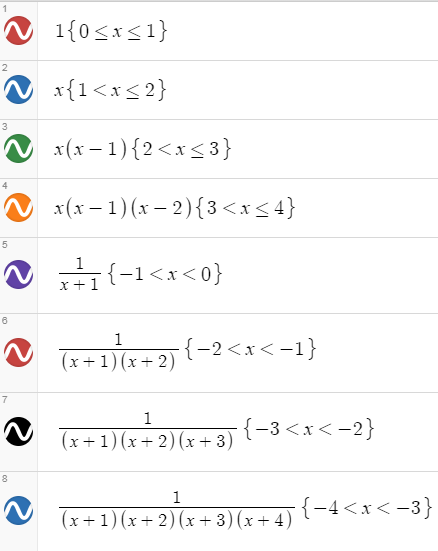
\includegraphics[scale=0.55]{Graph_values}
            
        }
    \end{homeworkSection}

\end{homeworkProblem}
\noindent
Notice that $h(x)$ satisfies $h(n)=n!$ and it is at least continuous for $x\geq0$, but it's piecewise definition and its many non-differentiable corners disqualify it from being out sought after factorial function. \textbf{One legitimate conclusion that arises out of this exercise is that $x!$, when we find it, will exhibit the same asymptotic behavior as $h$ at $x=-1,-2,-3,\ldots$, and thus won't be defined on the negative integers.}

\newpage

\begin{homeworkProblem}[\underline{Improper Riemann Integrals}]
    For reasons that will become clear, we need to make rigorous sense of an expression like 
    \[ \int_0^\infty e^{-t}dt .\]
    Most likely familiar from calculus, integrals over unbounded regions like $[0,\infty)$ are called \textit{improper Riemann integrals} and are defined by taking the limit of ``proper" integrals.
    \begin{homeworkSection}{Definition 8.4.3}
        Assume $f$ is defined on $[a,\infty)$ and integrable on every interval of the form $[a,b]$. then define $\int_a^\infty f$ to be
        \[ \lim_{b\to\infty}\int_a^bf ,\]
        provided the limit exists. In this case we say the improper integral $\int_a^\infty f$ \textit{converges}.
    \end{homeworkSection}
\end{homeworkProblem}

\begin{homeworkProblem}[8.4.9]
    \begin{homeworkSection}{(a)}
        Show that the improper integral $\int_a^\infty f$ converges $(\Leftarrow)$ if and $(\Rightarrow)$ only if, for all $\epsilon>0$ there exists $M>a$ such that whenever $d>c\geq M$ it follows that 
        \[ \left|\int_c^df\right|<\epsilon .\]
        (In one direction it will be useful to consider the sequence $a_n=\sum_a^{a+n}f$.)
        \sectionAnswer{
                $(\Leftarrow)$\\
            Assume that $\forall\ \epsilon>0,\ \exists\ M>a\ s.t.\ d>c\geq M \text{ implies } |\int_c^d f|<\epsilon$.\\
            \[ \lim_{b\to\infty}\int_a^b f \leq \lim_{b\to\infty}\left|\int_a^b f\right| = \left| \int_a^M f + \int_M^{b_1}f + \int_{b_1}^{b_2}f + \int_{b_1}^{b_2}f + \cdots \right| \]
            \[ \leq \left| \int_a^M f \right| + \left| \int_M^{b_1}f \right| + \left| \int_{b_1}^{b_2}f \right| + \left| \int_{b_1}^{b_2}f \right| + \cdots .\]
            By our assumption, each integral whose upper limit is $b_n$ amounts to be less than $\epsilon_n$ for any given positive $\epsilon_n$.
            \[ <L_1+\epsilon_1+\epsilon_2+\epsilon_3+\cdots = L+\sum_{n=1}^\infty\epsilon_n .\]
            So let $\epsilon_n = \frac{1}{2^n}$. Then:
            \[ L_1+\sum_{n=1}^\infty\epsilon_n=L_1\frac{\pi^2}{6}=L ,\]
            for some real $L$. Then, the integral $\int_a^\infty f$ converges.
        }
        \sectionAnswer{
                $(\Rightarrow)$\\
            Proof by Contradiction: Assume
            \[ \int_a^\infty f = L \And \exists\ \epsilon_1\ s.t.\ \forall\ M>a,\ d>c\geq M \And \left|\int_c^d f \right|\geq\epsilon_1 .\]
            So
            \[ \int_a^\infty=\int_a^M f + \int_{M=c_1}^{d_1} f + \int_{d_1=c_2}^d_2 f + \int_{d_2=c_3}^d_3 f + \cdots \]
            \[ \geq L_1+\epsilon_1+\epsilon_1+\epsilon_1+\cdots \]
            \[ = L_1+\sum_{n=1}^\infty \epsilon_1 = \infty\neq L \]
            for any real $L$.\\
            There is a contradiction, $\int_a^\infty f = L$ and $\int_a^\infty f \geq \infty$. Therefore the opposite is true.\\\\
            $\mathcal{QED}$
        }
    \end{homeworkSection}

    \begin{homeworkSection}{(b)}
        Show that if $0\leq f\leq g$ and $\int_a^\infty g$ converges then $\int_a^\infty f$ converges.
        \sectionAnswer{
            Considering the Riemann Sum Integral of g:
            \[ \int_a^c g
            = \lim_{b\to\infty}\sum+{k=1}^b\frac{c-a}{b}\cdot\sup_{[x_{k-1},x_k]}g
            = \lim_{b\to\infty}\sum+{k=1}^b\frac{c-a}{b}\cdot\inf_{[x_{k-1},x_k]}g
            .\]
            So the improper Riemann Sum:
            \[\lim_{c\to\infty}\int_a^c g
            = \lim_{c\to\infty}\lim_{b\to\infty}\sum_{k=1}^b\frac{c-a}{b}\cdot\sup_{[x_{k-1},x_k]}g
            = \lim_{c\to\infty}\lim_{b\to\infty}\sum_{k=1}^b\frac{c-a}{b}\cdot\inf_{[x_{k-1},x_k]}g
            .\]
            Similarly:
            \[\lim_{c\to\infty}\int_a^c f
            = \lim_{c\to\infty}\lim_{b\to\infty}\sum_{k=1}^b\frac{c-a}{b}\cdot\sup_{[x_{k-1},x_k]}f
            = \lim_{c\to\infty}\lim_{b\to\infty}\sum_{k=1}^b\frac{c-a}{b}\cdot\inf_{[x_{k-1},x_k]}f
            .\]
            Note, $\inf f \leq \sup g$ on any interval. So:
            \[ \lim_{c\to\infty}\lim_{b\to\infty}\sum_{k=1}^b\frac{c-a}{b}\cdot\inf_{[x_{k-1},x_k]}f\leq \lim_{c\to\infty}\lim_{b\to\infty}\sum_{k=1}^b\frac{c-a}{b}\cdot\sup_{[x_{k-1},x_k]}g = L \]
            \[ \lim_{c\to\infty}\int_a^c f \leq \lim_{c\to\infty}\int_a^c g = L \]
            \[ \lim_{c\to\infty}\int_a^c f \leq L .\]
            $\mathcal{QED}$
            
        }
    \end{homeworkSection}

\newpage

    \begin{homeworkSection}{(c)}
        Part (a) is a Cauchy criterion, and part (b) is a comparison test. State and prove an absolute convergence test for improper intergrals.
        \sectionAnswer{
            $\int f$ is absolutely convergent if $\int|f|$ converges.\\
            Assume $\int |f|$ converges. That is,
            \[ \forall\epsilon>0, \exists M\ s.t\ M\leq c<d \rightarrow\left|\int_c^d|f|\right|<\epsilon .\]
            Fix $M$ such that this holds.\\
            Show $\int_c^d f$ converges. That is, show
            \[ \forall\epsilon>0, \exists M\ s.t\ M\leq c<d \rightarrow \left|\int_c^d f\right|<\epsilon ?\]
            \[ -|f|\leq f\leq|f| \]
            \[ -\int_c^d|f|\leq\int_c^d f\leq\int_c^d|f| \]
            \[ \left|\int_c^d f\right|\leq \left|\int_c^d|f|\right|<\epsilon \]
            \[ \left|\int_c^d f\right|<\epsilon \]
            \(\mathcal{QED}\)
        }
    \end{homeworkSection}
    
\end{homeworkProblem}

\begin{homeworkProblem}[8.4.10]
    \begin{homeworkSection}{(a)}
        Use the properties of $e^t$ previously discussed to show
		$$ \int_0^\infty e^{-t}dt=1 .$$
		\sectionAnswer{
            Note, $[e^{-t}]'=-t^{-t}$.
            \[ \int_0^\infty e^{-t}dt = \int_0^\infty [-e^{-t}]'dt = -e^{-t}\bigg|^\infty_0 = -\frac{1}{e^\infty}+\frac{1}{e^0} = 0+\frac{1}{1} = 1 \]
            $\mathcal{QED}$
        }
    \end{homeworkSection}

\newpage

    \begin{homeworkSection}{$\star$\ (b)}
        Show
		\[ \frac{1}{\alpha}=\int_0^\infty e^{-\alpha t}dt, \text{ for all $\alpha>0$.} \]
		\sectionAnswer{
            \[ \frac{d}{dt}(e^{-\alpha t})=\frac{du}{dt}\frac{d}{du}e^u ,\]
            where $u=-\alpha t$, and so $du=-\alpha dt$, hence $\frac{du}{dt}=-\alpha$.
            \[ \frac{d}{dx}(e^{-\alpha t})=(-\alpha)e^u=-\alpha e^{-\alpha t} \]
            Therefore
            \[ \frac{\frac{d}{dt}(-e^{-\alpha t)}}{\alpha}=e^{-\alpha t} .\]
            And so:
            \[ \int_0^\infty e^{-\alpha t} dt = \frac{\int_0^\infty \frac{d}{dt}(-e^{-\alpha t}) dt}{\alpha} = \frac{-e^{-\alpha t}}{\alpha}\bigg|^\infty_0=\frac{\frac{1}{-e^{\alpha \infty}}-\frac{1}{-e^{\alpha 0}}}{\alpha}=\frac{\frac{1}{e^{\alpha 0}}-\frac{1}{e^{\alpha \infty}}}{\alpha}=\frac{\frac{1}{1}-\frac{1}{\infty}}{\alpha}=\frac{1-0}{\alpha}=\frac{1}{\alpha} \]
            $\mathcal{QED}$
        }
    \end{homeworkSection}

\end{homeworkProblem}

\noindent
    Just for a moment, let's take off our analysis gloves off and ask what we think might happen if we differentiate this formula with respect to $\alpha$.\\
    On the left: $\left[ \frac{1}{\alpha} \right]' = -\frac{1}{\alpha^2} $.\\
    On the right, let's brazenly crash through the integral sign and take the derivative of the integrand  $e^{-\alpha t}$ with respect to $\alpha$ (thinking of $t$ as a constant). The result is: \( \left[ e^{-\alpha t} \right]' = e^{-\alpha t}\cdot(-t) \).\\
    The question, then, is whether this was valid. That is, is it true that 
    \[ -\frac{1}{\alpha^2} = \int_0^\infty e^{-\alpha t}\cdot(-t) dt\ ?\]

\newpage

\begin{homeworkProblem}[8.4.11]
	\begin{homeworkSection}{(a)}
		Evaluate $\int_0^b te^{-\alpha t}dt$ using the integration-by-parts formula from exercise 7.5.6. The result will be an expression in $\alpha$ and $b$.
		\sectionAnswer{
		    Integration-by-parts: $\int fg' = fg - \int f'g$\\
		    $\int e^{-\alpha t}dt = \frac{-e^{-\alpha t}}{\alpha}+C$
			\[ \int_0^b \underset{\downarrow}{t}\cdot \overset{\uparrow}{e^{-\alpha t}}dt \]
			\[ = t\cdot\frac{-e^{-\alpha t}}{\alpha}\bigg|_0^b-\int_0^b\frac{-e^{-\alpha t}}{\alpha}dt = \frac{-1}{\alpha}(t\cdot e^{-\alpha t})\bigg|_0^b+\frac{1}{\alpha}\int_0^b e^{-\alpha t}dt \]
			\[ = \frac{1}{\alpha}\left( \int_0^be^{-\alpha t} dt - (t\cdot e^{-\alpha t})\bigg|_0^b \right) = \frac{1}{\alpha}\left( -\frac{e^{-\alpha t}}{\alpha}\bigg|_0^b - (t\cdot e^{-\alpha t})\bigg|_0^b \right) \]
		    \[ = \frac{1}{\alpha^2}\left( e^{-\alpha 0}-e^{-\alpha b}\right) - \frac{1}{\alpha}\left(b\cdot e^{-\alpha b}-0\cdot e^{-\alpha 0} \right) \]
			\[ = \frac{1}{\alpha^2}\left( 1-e^{-\alpha b}\right) - \frac{1}{\alpha}\left(b\cdot e^{-\alpha b} \right) \]
			$\mathcal{QED}$
		}
		\end{homeworkSection}
	
	\begin{homeworkSection}{(b)}
		Now compute $\int_0^\infty te^{-\alpha t}dt$ and verify this equation:
		\[ \frac{1}{\alpha^2}=\int_0^\infty te^{-\alpha t}dt \]
		\sectionAnswer{
			\[ \int_0^\infty te^{-\alpha t}dt = \lim_{b\to\infty}\frac{1}{\alpha^2}\left( 1-e^{-\alpha b}\right) - \frac{1}{\alpha}\left(b\cdot e^{-\alpha b} \right) \]
			Note, $\lim_{b\to\infty}b\cdot e^{-\alpha b}=0$, by Exercise 8.4.5. So 
			\[ = \frac{1}{\alpha^2}\left( 1-0 \right) - \frac{1}{\alpha}\left( 0 \right) = \frac{1}{\alpha^2} \]
			$\mathcal{QED}$
		}
		\end{homeworkSection}
	
\end{homeworkProblem}
\vspace{0.5cm}
\noindent
Yes, it holds: \(-\frac{1}{\alpha^2} = \int_0^\infty e^{-\alpha t}\cdot(-t) dt\).

\begin{homeworkProblem}[Definition 8.4.4 (Two-Variable Continuity)]
    A function $f:D\to\mathbb{R}$ is \textbf{continuous} at $(x_0,t_0)$ if for all $\epsilon>0$, there exists $\delta>0$ such that whenever $||(x,t)-(x_0,t_0)||<\delta$, it follows that 
    \[ |f(x,t)-f(x_0,t_0)|<\epsilon .\]
\end{homeworkProblem}

\begin{homeworkProblem}[8.4.12.]
	Assume the funtion $f(x,t)$ is continuous on the rectangle $D=\{(x,t):a\leq x\leq b, c\leq t\leq d\}$. Explain why the function
	\[ F(x)=\int_c^d f(x,t)dt \]
	is properly defined for all $x\in[a,b]$.

	\problemAnswer{
		$x\in[a,b]$, so $f(x,t)$ is continuous as long as $t\in[c,d]$. Note that the integral is from $c$ to $d$, so $f(x,t)$ in $F(x)$ is continuous. Certainly there are not uncountably many discontinuities in $f(x,t)$, so it's integrable (with respect to both $x$ and $t$), and $F(x)$ is well-defined.
	}
\end{homeworkProblem}

It should not be too surprising that Theorem 4.4.7 (Uniform Continuity on Compact Sets) has an analogue in the $\mathbb{R}^2$ setting. The set $D$ is compact in $\mathbb{R}^2$, and a continuous function on D is uniformly continuous in the sense that the $\delta$ can be chosen independently of a point $(x_0,t_0)$. 

\begin{homeworkProblem}[Theorem 8.4.5.]
    If $f(x,t)$ is continuous on $D$, then $F(x)=\int_c^d f(x,t)dt$ is uniformly continuous on $[a,b]$.
\end{homeworkProblem}

\begin{homeworkProblem}[8.4.13]
    Prove Theorem 8.4.5. above.
    
    \problemAnswer{
	    Assume $f(x,t)$ is continuous on $D$. So $\forall(x_0,t_0)\in D,\ \forall\epsilon>0,\ \exists\delta>0\ s.t.\ ||(x,t)-(x_0,t_0)||<\delta \rightarrow |f(x,t)-f(x_0,t_0)|<\epsilon.$\\
	    It must be shown that $\forall\epsilon>0,\ \exists\delta>0\ s.t.\ ||(x,t)-(x_0,t_0)||<\delta \rightarrow |F(x,t)-F(x_0,t_0)|<\epsilon, \forall(x_0,t_0)\in D.$\\
	    Assume $||(x,t)-(x_0,t_0)||<\delta$.\\
	    \[ |F(x,t)-F(x_0,t_0)| = \left|\int_c^d f(x,t)dt - \int_c^d f(x_0,t_0) dt\right| = \left|\int_c^d f(x,t)-f(x_0,t_0) dt\right| \overset{\triangle}{\leq} \int_c^d |f(x,t)-f(x_0,t_0)|dt \]
	    Note, $|f(x,t)-f(x_0,t_0)|<\epsilon_1$, by assumption. Let $\epsilon_1=\frac{d-c}{\epsilon}$.
	    \[ \int_c^d |f(x,t)-f(x_0,t_0)|dt < \int_c^d \epsilon_1 dt = (d-c)\epsilon_1 = \epsilon \]
	    $\mathcal{QED}$
    }
\end{homeworkProblem}

\noindent
As we were skeptical with the equation from 8.4.10-8.4.12; let's add the assumption that for each fixed value of $t$ in $[c,d]$, the function $f(x,t)$ is a differentiable function of $x$; that is,
\[ f_x(x,t)=\lim_{z\to x}\frac{f(z,t)-f(x,t)}{z-x} \]
exists for all $(x,t)\in D$. In addition, let's assume that the derivative function $f_x(x,t)$ is continuous. %%Why does this not go with the assumption that f is diffy?

\begin{homeworkSection}{Theorem 8.4.6.}
	If $f(x,t)$ and $f_x(x,t)$ are continuous on $D$, then the function $F(x)=\int_c^d f(x,t)dt$ is differentiable and
	\[ F'(x)=\int_c^df_x(x,t)dt .\]
	\textit{Proof.} Fix $x$ in $[a,b]$ and let $\epsilon>0$ be arbitrary. Our task is to find a $\delta>0$ such that 
	\[ \left| \frac{F(z)-F(x)}{z-x}-\int_c^d f_x(x,t)dt \right|<\epsilon \]
	whenever $0<|z-x|<\delta$.
\end{homeworkSection}

\begin{homeworkProblem}[8.4.14.]
    Finish the proof of Theorem $8.4.6.$ above

    \problemAnswer{
	    It was shown that if $f(x,t)$ is continuous on $D$, then $F(x)=\int_c^d f(x,t)dt$ is uniformly continuous on $[a,b]$, so $F(x)$ is also continuous. \\
	    Let $F_x(x)=\int_c^d f_x(x,t)dt$.\\
		Likewise, since $f_x(x,t)$ is continuous on $D$, $F_x(x)=\int_c^d f(x,t)dt$ is uniformly continuous on $[a,b]$, so $F_x(x)$ is also continuous.\\
		Consider $c\leq t\leq d$, since the integral in question is bounded as such.
        \[ \left| \frac{F(z)-F(x)}{z-x}-\int_c^d f_x(x,t)dt \right|\:
        =\:\left| \frac{\int_c^d f(x,t)dt - \int_c^df(z,t)dt}{z-x} - \frac{(z-x)\int_c^df_x(x,t)dt}{z-x} \right|
        \]
        \[
        =\:\left| \frac{\int_c^d f(x,t) - f(z,t) - (z-x)\frac{f(z,t)-f(x,t)}{z-x} dt}{z-x} \right|\:
        =\:\left| \frac{\int_c^d f(x,t) - f(z,t) - f(z,t)-f(x,t) dt}{z-x} \right|\:
        \]
        \[
        =\: \frac{2}{|z-x|}\left| \int_c^d f(x,t)-f(z,t)dt \right|\:
        \overset{\triangle}{\leq}
        \:\frac{2}{|z-x|} \int_c^d |f(x,t)-f(z,t)|dt
        =\:\frac{2}{|z-x|} |F(x)-F(z)|
        \]
        Note, $|z-x|<\delta$.\\
        Note, F(x) is continuous. So let $\epsilon_1$ be such that $|F(x)-F(z)|<\epsilon_1$, and $\delta$ such that $\epsilon_1=\frac{\delta\epsilon}{2}$. Then, 
        \[ \frac{2}{|z-x|} |F(x)-F(z)|\:
        <\: \frac{2}{|z-x|} \epsilon_1\:
        =\: \frac{2}{|z-x|} \frac{\delta\epsilon}{2}
        <\: \frac{2}{|z-x|} \frac{|z-x|\epsilon}{2}
        =\epsilon
        \]
        Therefore, $\left| \frac{F(z)-F(x)}{z-x}-\int_c^d f_x(x,t)dt \right|<\epsilon$, as desired.\\
        $\mathcal{QED}$
    }
\end{homeworkProblem}

\newpage

\begin{homeworkProblem}[\underline{Improper Integrals, Revisited}]
	\textbf{Theorem 8.4.6 is a formal justification for differentiating under the integral sign, but we need to extend this result to the case where the integral is improper.} Looking back one more time to our motivating example in this equation: $\frac{1}{\alpha}=\int_0^\infty e^{-\alpha t}dt, \text{ for all $\alpha>0$}$ ; we see that what we have is a function $f(x,t)$ where the domain of the variable $t$ is the unbounded interval $c\leq t<\infty$.\\
	Let's fix $x$ from some set $A\subseteq\mathbb{R}$. For such an $x$, we define
	\[ F(x)=\int_c^\infty f(x,t)dt=\lim_{d\to\infty}\int_c^d f(x,t)dt ,\]
	provided the limit exists.
	Notice that this is a \textit{pointwise} statement. Given an $x\in A$ and $\epsilon>0$, we can find an $M$ (perhaps dependent on $x$) where
	\[ \left| F(x)-\int_c^d f(x,t)dt \right|<\epsilon \]
	whenever $d\geq M$. \textbf{As we have seen on numerous occasions, the elixir required to ensure that good behaviour in the finite setting extends to the infinite setting is uniformity}.
	
	\begin{homeworkSection}{Definition 8.4.7.}
		Given $f(x,t)$ defined on $D=\{(x,t):x\in A,c\leq t\}$, assume $F(x)=\int_c^\infty f(x,t)dt$ exists for all $x\in A$. We say the improper integral \textit{converges uniformly} to $F(x)$ on $A$ if for all $\epsilon>0$, there exists $M>c$ such that
		\[ \left| F(x)-\int_c^df(x,t)dt \right|<\epsilon \]
		for all $d\geq M$ and all $x\in A$.
	\end{homeworkSection}
\end{homeworkProblem}

\begin{homeworkProblem}[8.4.15.]
	\begin{homeworkSection}{(a)}
		Show that the improper integral $\int_0^\infty e^{-xt}dt$ converges uniformly on the set $[1/2,\infty)$.
		\sectionAnswer{
			Show $\forall\epsilon>0, \exists M>c\ s.t.\ \left| \int_c^\infty e^{-xt}dt - \int_c^d e^{-xt}dt \right|<\epsilon, \forall d\geq M, \forall x\in[1/2,\infty)$.
			\[ \left| \int_c^\infty e^{-xt}dt - \int_c^d e^{-xt}dt \right| = \left| \frac{1}{x} - \int_0^d e^{-xt}dt \right| = \left| \frac{1}{x} - \frac{-e^{-xt}}{x}\bigg|_0^d \right| = \left| \frac{1}{x} + [\frac{e^{-xd}}{x}-\frac{e^{-x0}}{x}] \right| = \frac{e^{-xd}}{x} \]
			\[ = \frac{1}{xe^{dx}} \leq \frac{1}{xe^{Mx}}\overset{?}{<}\epsilon \]
			Let $M>2\log\frac{1}{\epsilon}$. Then:
			\[ M>2\log\frac{1}{\epsilon}>\frac{\log\frac{1}{\epsilon}}{x}>\frac{\log\frac{1}{\epsilon}}{x}-\frac{\log x}{x}=\frac{\log(\frac{1}{\epsilon}/x)}{x} \]
			\[ \log(\frac{1}{\epsilon}/x)<Mx\ \rightarrow\ \frac{\frac{1}{\epsilon}}{x}<e^{Mx}\ \rightarrow\ \frac{1}{xe^{Mx}}<\epsilon .\]
			$\mathcal{QED}$
		}
	\end{homeworkSection}

	\begin{homeworkSection}{(b)}
		Is the convergence uniform on $(0,\infty)$?
        \sectionAnswer{
            No, $\lim_{x\to0^+}\Rightarrow\frac{1/\epsilon}{x}\to\infty\not< M$
        }
    \end{homeworkSection}
\end{homeworkProblem}

\begin{homeworkProblem}[8.4.16.]
	Prove the following analogue of the Weierstrass M-Test for improper integrals:\\
	If $f(x,t)$ satisfies $|f(x,t)|\leq g(t)$ for all $x\in A$ and $\int_a^\infty g(t)dt$ converges, then $\int_a^\infty f(x,t)dt$ converges uniformly on $A$.

	\problemAnswer{
	    
		Using the Cauchy definition of convergence, we know: $\forall\epsilon>0,\exists M>a\ s.t.\ M\leq c<d \rightarrow \left|\int_c^d g(t) dt\right|<\epsilon$.\\
		It must be shown that for all $\epsilon>0$, there exists $M>c$ such that $\left| F(x)-\int_a^df(x,t)dt \right|<\epsilon$
		\[ \left|\int_a^d f(x,t)dt\right|\overset{\triangle}{\leq}\int_a^d |f(x,t)|dt\leq \int_a^d g(t)dt,\ \forall x\in A \]
		Since $\int g(t) dt$ converges, given any $\epsilon_1$ $\int_a^d g(t)dt<\epsilon_1,\ \forall x\in A$. Therefore:
		\[ \left|\int_a^d f(x,t)dt\right|<\epsilon_1,\ \forall x\in A \]
		\[ \left| F(x)-\int_c^df(x,t)dt \right|\ 
		=\ \left| \int_a^\infty f(x,t)dt-\int_a^df(x,t)dt \right|\ 
		=\ \left| \int_d^\infty f(x,t)dt \right| \] 
		\[ =\ \left| \int_d^{d_1} f(x,t)dt + \int_{d_1}^{d_2} f(x,t)dt + \cdots+  \int_{d_{n-1}}^{d_n} f(x,t)dt + \cdots \right| \]
		\[
		\overset{\triangle}{\leq} \left| \int_d^{d_1} f(x,t)dt \right| + \left| \int_{d_1}^{d_2} f(x,t)dt \right| + \cdots + \left| \int_{d_{n-1}}^{d_n} f(x,t)dt \right| + \cdots
		\]
		Note that all $d_n$ are greater than $a$. So each piece $\left|\int_{d_{n-1}}^{d_n} f(x,t)dt\right|<\epsilon_n,\ \forall x\in A$, given any $\epsilon_n$.
		\[ <\epsilon_1+\epsilon_2+\cdots+\epsilon_n+\cdots = \sum_{n=1}^\infty \epsilon_n \]
		Let $\epsilon_n=\frac{6\epsilon}{\pi^2 n}$. Then:
		\[ \sum_{n=1}^\infty \epsilon_n = \sum_{n=1}^\infty \frac{6\epsilon}{\pi^2 n} = \frac{\pi^2 6\epsilon}{6 \pi^2}=\epsilon \]
		So 
		\[ \left| F(x)-\int_c^df(x,t)dt \right|<\epsilon \]
		$\mathcal{QED}$
	}
\end{homeworkProblem}\\

An immediate consequence of Definition 8.4.7 is that if the improper integral converges uniformly then the sequence of functions defined by 
\[ F_n(x)=\int_c^{c+n} f(x,t)dt \]
converges uniformly to $F(x)$ on $[a,b]$. \textbf{This observation gives us access to the host of useful results we developed from Chapter 6 (Sequences and Series of Functions)}.

\begin{homeworkProblem}[Theorem 8.4.8.]
	If $f(x,t)$ is continuous on $D=\{(x,t):a\leq x\leq b, c\leq t\}$, then
	\[ F(x)=\int_c^\infty f(x,t)dt \]
	is uniformly continuous on $[a,b]$, provided the integral converges uniformly. 
\end{homeworkProblem}

\begin{homeworkProblem}[8.4.17.]
	Prove Theorem 8.4.8, above.
	
	\problemAnswer{
    	It must be shown that $\forall\epsilon>0,\ \exists\delta>0\ s.t.\ |x_0-x|<\delta\ \rightarrow\ |F(x_0)-F(x)|<\epsilon$\\
    	Fix $\epsilon>0$ arbitrarily, and assume $|x_0-x|<\delta$.\\
    	Note, since $t$ is constant in $F(x)$, $|x_0-x|<\delta\ \rightarrow\ ||(x_0,t_0)-(x,t)||<\delta$.\\
    	Considering $|F(x)|$:
    	\[ |F(x)|\ 
    	=\ \left| F(x) + \int_c^df(x,t)dt - \int_c^df(x,t)dt \right|\ 
    	\overset{\triangle}{\leq}\ \left| F(x) - \int_c^df(x,t)dt \right| + \left| \int_c^df(x,t)dt \right|
    	<\epsilon_1+\left| \int_c^df(x,t)dt \right|
    	, \]
    	for any $\epsilon_1$, by the fact that $F(x)$ converges uniformly.
    	\[ |F(x_0)-F(x)|\ 
    	=\ |F(x_0)+(-F(x))|\ 
    	\overset{\triangle}{\leq}\ |F(x_0)|+|F(x)|\ 
    	<\ \epsilon_1+\left| \int_c^df(x_0,t)dt \right| + \epsilon_1+\left| \int_c^df(x,t)dt \right|
    	\]
    	\[
    	\overset{\triangle}{\leq}\ 2\epsilon_1 + \int_c^d |f(x_0,t)| dt + \int_c^d |f(x,t)| dt\ 
    	=\ 2\epsilon_1 \int_c^d |f(x_0,t)| - |f(x,t)| dt\ 
    	\overset{\triangledown}{\leq}\ 2\epsilon_1 + \int_c^d |f(x_0,t) - f(x,t)| dt
    	\]
    	\[
    	<2\epsilon_1 + \int_c^d \epsilon_2 dt
    	,\]
    	for any $\epsilon_2$, by the continuity of $f(x,t)$.
    	\[ =\ 2\epsilon_1 + (d-c)\epsilon_2 \]
    	So let $\epsilon_1=\frac{\epsilon}{4}$, and let $\epsilon_2 = \frac{\epsilon}{2(d-c)}$. Then:
    	\[ =\frac{\epsilon}{2} + \frac{\epsilon}{2} = \epsilon .\]
    	$\mathcal{QED}$
	}
\end{homeworkProblem}

\begin{homeworkProblem}[Theorem 8.4.9.]
	Assume the function $f(x,t)$ is continuous on $D=\{(x,t):a\leq x\leq b, c\leq t\}$ and $F(x)=\int_c^\infty f(x,t)dt$ exists for each $x\in[a,b]$. If the derivative function $f_x(x,t)$ exists and is continuous, then
	\[ F'(x)=\int_c^\infty f_x(x,t)dt ,\]
	provided this integral converges uniformly.
\end{homeworkProblem}

\begin{homeworkProblem}[8.4.18.]
	Prove Theorem 8.4.9, above.
	
	\problemAnswer{
		It must be shown that $\forall\epsilon>0,\ \exists\delta>0\ s.t.\ |z-x|<\delta\ \rightarrow\ \left| \frac{F(z)-F(x)}{z-x}-\int_c^\infty f_x(x,t)dt \right|<\epsilon$.\\
		Fix $\epilson>0$ arbitrarily, and assume $|z-x|<\delta$.\\
		Note, since $t$ is constant in $F(x)$, $|z-x|<\delta\ \rightarrow\ ||(z,t_0)-(x,t)||<\delta$.\\
			Considering $|F(x)|$:
    	\[ |F(x)|\ 
    	=\ \left| F(x) + \int_c^df(x,t)dt - \int_c^df(x,t)dt \right|\ 
    	\overset{\triangle}{\leq}\ \left| F(x) - \int_c^df(x,t)dt \right| + \left| \int_c^df(x,t)dt \right|
    	<\epsilon_1+\left| \int_c^df(x,t)dt \right|
    	, \]
    	for any $\epsilon_1$, by the fact that $F(x)$ converges uniformly.
    	
    	\[ \left| \frac{F(z)-F(x)}{z-x}-\int_c^\infty f_x(x,t)dt \right|\:
        =\:\left| \frac{\int_c^\infty f(x,t)dt - \int_c^\infty f(z,t)dt}{z-x} - \frac{(z-x)\int_c^\infty f_x(x,t)dt}{z-x} \right|
        \]
        \[
        =\:\left| \frac{\int_c^\infty f(x,t) - f(z,t) - (z-x)\frac{f(z,t)-f(x,t)}{z-x} dt}{z-x} \right|\:
        =\:\left| \frac{\int_c^\infty f(x,t) - f(z,t) - f(z,t)-f(x,t) dt}{z-x} \right|\:
        \]
        \[
        =\: \frac{2}{|z-x|}\left| \int_c^\infty f(x,t)-f(z,t)dt \right|\:
        \overset{\triangle}{\leq}
        \:\frac{2}{|z-x|} \int_c^\infty |f(x,t)-f(z,t)|dt
        =\:\frac{2}{|z-x|} |F(x)-F(z)|
        \]
        Note, $|z-x|<\delta$.\\
        Note, F(x) is continuous. So let $\epsilon_1$ be such that $|F(x)-F(z)|<\epsilon_1$, and $\delta$ such that $\epsilon_1=\frac{\delta\epsilon}{2}$. Then, 
        \[ \frac{2}{|z-x|} |F(x)-F(z)|\:
        <\: \frac{2}{|z-x|} \epsilon_1\:
        =\: \frac{2}{|z-x|} \frac{\delta\epsilon}{2}
        <\: \frac{2}{|z-x|} \frac{|z-x|\epsilon}{2}
        =\epsilon
        \]
        Therefore, $\left| \frac{F(z)-F(x)}{z-x}-\int_c^d f_x(x,t)dt \right|<\epsilon$, as desired.\\
        $\mathcal{QED}$
	}
\end{homeworkProblem}

\newpage

\begin{homeworkProblem}[\underline{The Factorial Function}]
	It's time to return our attention to the equation from earlier in this section:
	\[ \frac{1}{\alpha}=\int_0^\infty e^{-\alpha t}dt, \text{ for all }\alpha>0 .\]
\end{homeworkProblem}

\begin{homeworkProblem}[8.4.19.]
	\begin{homeworkSection}{(a)}
		Although we verified it directly, show how to use the theorems in this section to give a second justification for the formula
		\[ \frac{1}{\alpha^2}=\int_0^\infty te^{-\alpha t}dt, \text{ for all }\alpha>0 .\]
		\sectionAnswer{
			\[ \frac{1}{\alpha} = \int_0^\infty e^{-\alpha t} dt \]
			\[ \left[\frac{1}{\alpha}\right]' = \left[\int_0^\infty e^{-\alpha t} dt\right]' \]
			\[ -\frac{1}{\alpha^2} = \int_0^\infty \left[e^{-\alpha t}\right]' dt = \int_0^\infty-t^{-\alpha t}dt .\]
			Therefore
			\[ \frac{1}{\alpha} = \int_0^\infty te^{-\alpha t} dt \]
			$\mathcal{QED}$
		}
	\end{homeworkSection}

\newpage

	\begin{homeworkSection}{(b)}
		Now derive the formula
		\[ \frac{n!}{\alpha^{n+1}}=\int_0^\infty t^ne^{-\alpha t}dt, \text{ for all }\alpha>0 .\]
        \sectionAnswer{
		    Note, $\frac{1}{\alpha}$ is infinitely differentiable with respect to $\alpha$:
		    \[ \left[\frac{1}{\alpha}\right]^{(n)}= 
		    \left\{
		    \begin{array}{cc}
                \frac{n!}{\alpha^{n-1}}& n\text{ even} \\
		        -\frac{n!}{\alpha^{n-1}}& n\text{ odd}
		    \end{array}
		    \right.
		    .\]
		    Similarly, $e^{-\alpha t}$ is infinitely differentiable with respect to $\alpha$: $\frac{d}{d\alpha}e^{-\alpha t}=-t\cdot e^{-\alpha t}$. And so,
		    \[ \left[\int_0^\infty te^{-\alpha t} dt\right]^{(n)} = \int_0^\infty \left[te^{-\alpha t}\right]^{(n)} dt=
		    \left\{
		    \begin{array}{cc}
                \int_0^\infty t^ne^{-\alpha t}dt& n\text{ even} \\
		        -\int_0^\infty t^ne^{-\alpha t}dt& n\text{ odd}
		    \end{array}
		    \right.
		    \]
		    Since the negatives of each side correspond to the same parity of $n$,
		    \[ \frac{n!}{\alpha^{n-1}} = \int_0^\infty t^ne^{-\alpha t}dt \]
		    $\mathcal{QED}$
	    }
	\end{homeworkSection}
\end{homeworkProblem}

If we set $\alpha=1$ in this equation, we (finally) get
\[ n!=\int_0^\infty t^ne^{-t}dt .\]
\textbf{The appearance of $n!$ on the left side of this equation is exciting, especially because where $n$ appears on the right it can be meaningfully replaced by a real variable $x$, at least when $x\geq 0$. This is the equation we have been looking for!}

\newpage

\begin{homeworkProblem}[Definition 8.4.10]
	For $x\geq0$, define the factorial function
	\[ x!=\int_0^\infty t^xe^{-t}dt .\]
\end{homeworkProblem}

\begin{homeworkProblem}[8.4.20.]
	\begin{homeworkSection}{(a)}
		$(i)$ Show that $x!$ is an infinitely differentiable function on $(0,\infty)$ and $(ii)$ produce a formula for the $n^{\text{th}}$ derivative. $(iii)$ In particular, show that $(x!)''>0$.
		\sectionAnswer{
			    $(i)(ii)$ 
			    $x!= \int_0^\infty t^xe^{-t}dt$. When we take the derivative, we take it with respect to x. So the first derivative of this would be \[ x!' = \left[\int_0^\infty t^xe^{-t}dt \right]'=
			    \int_0^\infty\left[ t^xe^{-t} \right]'dt= \int_0^\infty \left[ t^x \right]'e^{-t}dt.\]
			    So \[ e^{-t}[t^x]' = e^{-t}\ln(t) t^x ,\] 
			    \[ e^{-t}[t^x]''= e^{-t}\ln(t)\ln(t) t^x... \]
			    \[ e^{-t}[t^x]^{(n)}= e^{-t}\big[\ln(t)\cdot ln(t)\underset{n\text{ times}}{\cdots} \ln(t)\big] t^x= e^{-t}\ln(nt)t^x \]
			    For all n, this works, therefore it is infinitely differentiable.\\
	    		$(iii)$
	    	\[ (x!)'' = \int_0^\infty\left[ t^xe^{-t} \right]''dt = \int_0^\infty\left[ t^x \right]''e^{-t}dt = \int_0^\infty e^{-t}\ln(2t)t^x dt \]
	    	Note, $e^{-t}$, $\ln(2t)$, and $t^x$ are all nonnegative terms when $t\geq 0$. So the product of these nonnegative factors is nonnegative, thus the function is nonnegative and so it's integral is nonnegative as well. 
	    	%$[t^x]''= e^{-t}ln(2t)t^x$
		}
	\end{homeworkSection}
		\begin{homeworkSection}{(b)}
		Use the integration-by-parts formula employed earlier to show that $x!$ satisfies the functional equation
		\[ (x+1)!=(x+1)x! \]
		\sectionAnswer{
			\[ (x+1)! = \int_0^\infty t^{x+1}e^{-t} dt
			= t^{x+1}e^{-t}\bigg|_0^\infty + \int_0^\infty(x+1)t^x e^{-t}dt
			\]
			\[
			= t^{x+1}e^{-t}\bigg|_0^\infty + (x+1)\int_0^\infty t^x e^{-t}dt
			= t^{x+1}e^{-t}\bigg|_0^\infty+(x+1)x!
			= 0+(x+1)x!=(x+1)x!
			\]
			$\mathcal{QED}$
		}
	\end{homeworkSection}
\end{homeworkProblem}

The previous exercise is our first piece of evidence that we have found the right definition for $x!$. There's more to come.

A consequence of $(x!)''>0$ is that $x!$ is a \textit{convex} function. In calculus, this is usually referred to as ``concave up" and means that the line segment connecting two points on the graph of $x!$ always sits above the curve. Said another way, there are no inflection points in $x!$ and the slope of the curve steadily increases as the graph passes through the points $(n,n!)$ for $n=0,1,2,\ldots$. We did not mention this property at the time, but reflecting on our earlier analogy between $2^x$ and $x!$, convexity is a natural condition to desire in out factorial function.

In fact, not only is $x!$ convex, but $\log(x!)$ is also convex. This is a stronger statement. (Consider for instance, the graphs of $x^2+1$ and $\log(x^2+1)$.) The proof is a little technical and we won't go through it, %whew
but the fact that $\log(x!)$ is convex on $x\geq0$ is quite significant. Here's why.

\begin{homeworkProblem}[Theorem 8.4.11. (Bohr-Mollerup Theorem)]
    There is a unique positive function $f$ defined on $x\geq0$ satisfying
    \renewcommand{\labelenumi}{(\roman{enumi})}
    \begin{enumerate}
        \item $f(0)=1$
        \item $f(x+1)=(x+1)f(x)$, and 
        \item $\log(f(x))$ is convex.
    \end{enumerate}
    \noindent
    Because $x!$ satisfies all these properties, it follows that $f(x)=x!$.\\\\
    \textit{Proof.}\\
    We need one more geometrically plausible fact about convex functions. If $[a,b]$ and $[a',b']$ are two intervals in the domain of a convex function $\phi$, and $a\leq a'$ and $b\leq b'$, then the slopes of the chords over these intervals satisfy
    \[ \frac{\phi(b)-\phi(a)}{b-a}\leq\frac{\phi(b')-\phi(a')}{b'-a'} .\]
    Because $f$ satisfies properties (i) and (ii) we know $f(n)=n!$ for all $n\in\mathbb{N}$.\\
    \textbf{Now fix $n\in\mathbb{N}$ and $x\in(0,1]$.}
\end{homeworkProblem}

\newpage

\begin{homeworkProblem}[8.4.21.]
    \begin{homeworkSection}{(a)}
        Use the convexity of $\log(f(x))$ and the three intervals $[n-1,n];\ [n,n+x];\ [n,n+1]$ to show 
        \[ x\log(n)\leq\log(f(n+x))-\log(f(n))\leq x\log(n+1) .\]
        \sectionAnswer{
            Recall the second part of the Bohr-Mollerup Theorem: \( f(x+1)=(x+1)f(x) .\)\\
            Note, \(n-1<n<n+x\leq n+1\). So, using the convexity of $\log(f(x))$:
            \[ \frac{\log(f(n))-\log(f(n-1))}{n-(n-1)}
            \leq \frac{\log(f(n+x))-\log(f(n))}{n+x-n}
            \leq \frac{\log(f(n+1))-\log(f(n))}{n+1-n} \]
            
            \[ \log(nf(n-1))-\log(f(n-1))
            \leq \frac{\log(f(n+x))-\log(f(n))}{x}
            \leq \log((n+1)f(n))-\log(f(n)) \]
            
            \[ \log(n)+\log(f(n-1))-\log(f(n-1))
            \leq \frac{\log(f(n+x))-\log(f(n))}{x}
            \leq \log(n+1)+\log(f(n))-\log(f(n)) \]
            
            \[ \log(n)
            \leq \frac{\log(f(n+x))-\log(f(n))}{x}
            \leq \log(n+1) \]
            
            \[ x\log(n)
            \leq \log(f(n+x))-\log(f(n))
            \leq x\log(n+1) \]
            $\mathcal{QED}$
        }
    \end{homeworkSection}

    \begin{homeworkSection}{(b)}
        Show $\log(f(n+x))=\log(f(x))+\log\big((x+1)(x+2)\cdots(x+n)\big)$.
        \sectionAnswer{
            Recall the second part of the Bohr-Mollerup Theorem: \( f(x+1)=(x+1)f(x) .\) So:
            \[ f(n+x)=f(x+n)=(x+1)f(x+(n-1)) \]
            \[ f(x+(n-1))=(x+(n-1))f(x+(n-2)) \]
            \[ f(x+(n-2))=(x+(n-2))f(x+(n-3)) \]
            Generally, \( f(x+(n-k))=(x+(n-k))f(x+(n-k-1)) \). So putting these together:
            \[ f(n+x) = (x+n)(x+(n-1))(x+(n-2))\cdots(x+1)f(x+(n-n)) = (x+1)(x+2)\cdots(x+n)f(x) .\]
            Simply using the $\log$ product rule:
            \[ \log(f(n+x)=\log(f(x))+\log((x+1)(x+2)\cdots(x+n)) \]
            $\mathcal{QED}$
        }
    \end{homeworkSection}

\newpage

    \begin{homeworkSection}{(c)}
        Now establish that 
        \[ 0\leq\log(f(x))-\log\left( \frac{n^xn!}{(x+1)(x+2)\cdots(x+n)} \right)\leq x\log(1+\frac{1}{n}) .\]
        \sectionAnswer{
            Considering $\log(f(n+x))-\log(n!)$:
            \[ 
            \log(f(n+x))-\log(n!)
            = \log(f(x))+\log((x+1)(x+2)\cdots(x+n))-\log(n!)
            \]
            \[
            = \log(f(x))-\left[ \log(n!) - \log\left( (x+1)(x+2)\cdots(x+n) \right) \right]
            = \log(f(x))-\log\left( \frac{n!}{(x+1)(x+2)\cdots(x+n)} \right)
            .\]
            Considering $x\log(1+n)$:
            \[ 
            x\log(1+n)=x\log\left( \frac{1+n}{n} \right) + x\log(n)=x\log\left( 1+\frac{1}{n} \right) + x\log(n)
            .\]
            So considering the inequality shown in part (a) above:
            \[ x\log(n) \leq \log(f(n+x))-\log(f(n)) \leq x\log(n+1) \]
            \[ x\log(n) \leq \log(f(x))-\log\left( \frac{n!}{(x+1)(x+2)\cdots(x+n)} \right) \leq x\log\left( 1+\frac{1}{n} \right) + x\log(n) \]
            \[ x\log(n) - x\log(n) \leq \log(f(x))-\log\left( \frac{n!}{(x+1)(x+2)\cdots(x+n)} \right) - x\log(n) \leq x\log\left( 1+\frac{1}{n} \right) \]
            \[ 0 \leq \log(f(x))-\log\left( \frac{n!}{(x+1)(x+2)\cdots(x+n)} + x\log(n) \right)  \leq x\log\left( 1+\frac{1}{n} \right) \]
            Note, $x\log(n)=\log(n^x)$. So:
            \[ 0 \leq \log(f(x))-\log\left( \frac{n^x n!}{(x+1)(x+2)\cdots(x+n)} \right)  \leq x\log\left( 1+\frac{1}{n} \right) \]
            $\mathcal{QED}$
        }
    \end{homeworkSection}
    
\newpage
    
    \begin{homeworkSection}{(d)}
        Conclude that 
        \[ f(x)=\lim_{n\to\infty}\frac{n^xn!}{(x+1)(x+2)\cdots(x+n)}, \text{ for all } x\in(0,1] .\]
        \sectionAnswer{
            Consider the limit of the inequality shown in part (c) above:
            \[ \lim_{n\to\infty}0 \leq \log(f(x))-\log\left( \frac{n^x n!}{(x+1)(x+2)\cdots(x+n)} \right)  \leq x\log\left( 1+\frac{1}{n} \right) \]
            \[ =\lim_{n\to\infty}0 \leq \log(f(x))-\log\left( \frac{n^x n!}{(x+1)(x+2)\cdots(x+n)} \right)  \leq x\log\left( 1 \right) \]
            \[ =\lim_{n\to\infty}0 \leq \log(f(x))-\log\left( \frac{n^x n!}{(x+1)(x+2)\cdots(x+n)} \right)  \leq 0 \]
            So by Squeeze Theorem:
            \[ \lim_{n\to\infty} \log(f(x))-\log\left( \frac{n^x n!}{(x+1)(x+2)\cdots(x+n)} \right)=0 \]
            \[ \log(f(x)) = \lim_{n\to\infty} \log\left( \frac{n^x n!}{(x+1)(x+2)\cdots(x+n)} \right) \]
            \[ f(x) = \lim_{n\to\infty} \left( \frac{n^x n!}{(x+1)(x+2)\cdots(x+n)} \right) \]
            $\mathcal{QED}$
        }
    \end{homeworkSection}
    
    \begin{homeworkSection}{(e)}
        Finally, show that the conclusion in (d) holds for all $x\geq0$.
        
        \sectionAnswer{
            Note that without loss of generality, if $x>1$, it can be expressed as $x=m+x_1$, where $m\in\mathbb{N}$,and $x_1\in(0,1]$. And since what was shown in parts (a), (b), and (c) was for any $n_1\in\mathbb{N}$, let $n_1=n+m$; similar to a proof by induction.\\
            $\mathcal{QED}$
        }
    \end{homeworkSection}
    
    
    Because we have arrived at an explicit formula for $f(x)$, the function $f(x)$ must be unique. By virtue of the fact that $x!$ satisfies conditions (i), (ii), and (iii) of the theorem, we can conclude that $x!$ is this unique function; i.e., $f(x)=x!$. Thus, not only have we proved the theorem, but we have also discovered an alternate representation for the factorial function called the \textit{Gauss product formula}:
    \[ x! = \int_0^\infty t^xe^{-t}dt = \lim_{n\to\infty}\frac{n^xn!}{(x+1)(x+2)\cdots(x+n)} ,\]
    for all $x\geq0$.
\end{homeworkProblem}\\

What happens when $x<0$? The integral $\int_0^\infty t^xe^{-t}dt$ in Definition 8.4.10 becomes improper for a second reason when $x<0$ because $t^x$ is unbounded and undefined at $t=0$. If $-1<x<0$, it is not hard to show that the integral still converges. On the other hand, the functional equation in Exercise 8.4.20(b) provides a natural way to extend the definition of $x!$ to all of $\mathbb{R}$. Just as in Exercise 8.4.8, the resulting function is never zero, alternating between positive and negative components with vertical asymptotes at $x=-1,-2,-3,\ldots$. 

\homeworkProblem[\underline{The Gamma Function}]
The focus of our discussion has been on the ingredients that go into the definition of $x!$ - improper integrals, proper definitions of exponential functions, differentiating under the integral sign - but the end result is a function worthy of its own seperate chapter. Since its deiscovery by Euler, the factorial function has become ubiquitous in numerous branches of analysis.

One of the early modifications that occured was a shift in the domain of $x!$ and a change in the notation. Adrien Marie Legendre introduced the Greek letter $\Gamma$ (gamma) and set
\[ \Gamma(x)=(x-1)!=\int_0^\infty t^{x-1}e^{-t}dt ,\]
so that $\Gamma(n+1)=n!$ and $x\Gamma(x)=\Gamma(x+1)$. This convention eventually became the standart, and so it is the gamme function that routinely appears in formulas from number theory, probability, geometry, and beyond. 

Philip Davis's article on the history of the gamma function is an excellent place to get a sense of the important role the gamma function has played in the development of analysis. Davis's essay seems to be at least part of the inspiration for a wonderful series of articles by David Fowler that explore the properties of $x!$ in an original and accessible way. Here is one of the anecdotes Fowler offers, which serves as an enticing clue for how intricately the gamma/factorial function is connected to the larger mathematical landscape.\\


Recall that when $x!$ is extended to all of $\mathbb{R}$ via the functional equation $x!=x(x-1)!$ we get asymptotes and every negative integer. Thus, there is a compelling reason to consider the reciprocal function $1/x!$ which we can take to be zero for $x=\{-1,-2,-3,\cdots\}$


\begin{homeworkProblem}[8.4.22.]
    \begin{homeworkSection}{(a)}
        Where does $g(x)=\frac{x}{x!(-x)!}$ equal zero? What other familiar function has the same set of roots?
        
        \sectionAnswer{
        %$g(x)=\frac{x}{x!(-x)!}$\\
        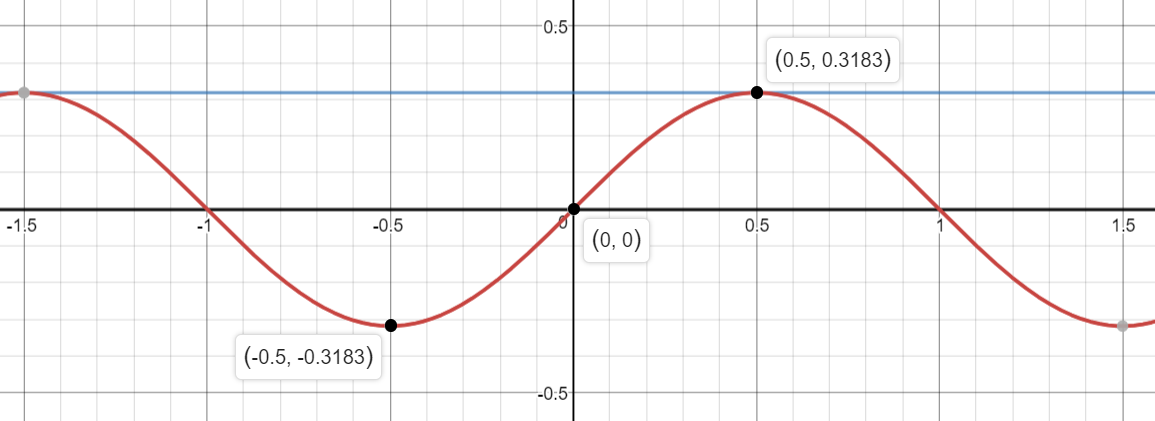
\includegraphics[scale=0.5]{ANALYSIS}
        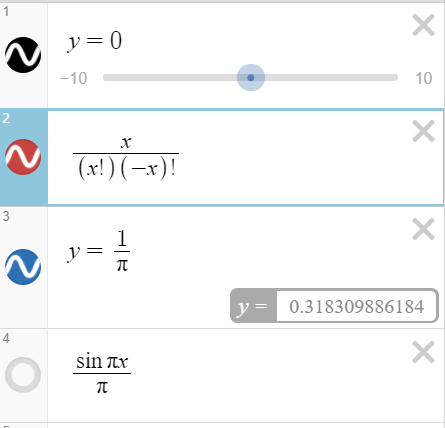
\includegraphics[scale=0.4]{Analysis_yx}
        $g(x)$ has roots at every integer, like $\sin(\pi x)$. It also looks like $\sin(\pi x)$, with $\min$ and $\max$ values to $\frac{1}{\pi}$ and $-\frac{1}{\pi}$. Graphically, $g(x)$ matches up perfectly with $\frac{\sin(\pi x)}{\pi}$ (not shown above). 
        }
    \end{homeworkSection}
    
\newpage
    
    \begin{homeworkSection}{(b)}
        The function $e^{-x^2}$ provides the raw material for the all-important Gaussian bell curve from probability, where it is known that $\int_{-\infty}^\infty e^{-x^2}dx=\sqrt\pi$. Use this fact (and some standard integration techniques) to evaluate $(1/2)!$.
        
        \sectionAnswer{
        \[ x!=\int_{0}^\infty t^{x}e^{-t}dt \]
        \[ (\frac{1}{2})!=\int_{0}^\infty \sqrt{t}e^{-t}dt\]
        By using integration by parts, we get $u=\sqrt{t}, du=\frac{1}{2\sqrt{t}}dt$ and $dv=e^{-t}, v=-e^{-t}$.
        So, \[ \int_{0}^\infty \sqrt{t}e^{-t}dt= -\sqrt{t}e^{-t}-\int_{0}^\infty \frac{-e^{-t}}{2\sqrt{t}}dt \]
        By using w-substitution, we get $w=\sqrt{t} \rightarrow w^{2}=t$, and $dw=\frac{1}{2\sqrt{t}}dt$. With this w-substitution our bounds remain the same. 
        Thus, \[ =-\sqrt{t}e^{-t}-\int_{0}^\infty-e^{u^{2}}du \] \[ =-\sqrt{t}e^{-t}+\int_{0}^\infty e^{-t^{2}}dt \]
        Now, evaluating $-\sqrt{t}e^{-t}\bigg|_{0}^\infty$, we get $\sqrt{\infty}e^{-\infty}=\frac{\sqrt{\infty}}{e^{\infty}}\Rightarrow \frac{\infty}{\infty}$. By L'Hospital's rule,
        \[ =\frac{-\frac{1}{2}t^\frac{-1}{2}}{e^t}=-\frac{1}{2}\frac{1}{t^{\frac{1}{2}}e^t}=-\frac{1}{2\infty^\frac{1}{2}e^\infty} \Rightarrow 0.\]  
        Looking at $\int_{0}^\infty e^{-t^{2}}dt$, we have that $\int_{-\infty}^\infty e^{-t^{2}}dt = \sqrt{\pi}$. Since the $t$ in $e^{-t{^2}}$ is not affected by the sign of t itself (it's squared), we can say 
        \[ \int_{-\infty}^\infty e^{-t^{2}}dt= 2\int_{0}^\infty e^{-t^{2}}dt=\frac{\sqrt{\pi}}{2} \].
        }
    \end{homeworkSection}

    \begin{homeworkSection}{(c)}
        Now use (a) and (b) to conjecture a striking relationship between the factorial function and a well-known function from trigonometry.
        
        \sectionAnswer{
        \[ \frac{x}{x!(-x)!} = \frac{\sin(\pi x)}{\pi} \]
        The factorial function can be composed in such a way that it's very similar to the sine function. It's roots however are at every integer, so it fits $\sin(\pi x)$. Also, instead of going in the y direction from $(-1,1)$, it's mix and max is $(\frac{-1}{\pi}, \frac{1}{\pi})$.\\
        Perhaps other trigonometric functions can also be defined using the Gamma function, and vice-versa. This would also give reason to believe the gamma function may be expressed as a Fourier Series?
        }
    \end{homeworkSection}
\end{homeworkProblem}

\newpage

\begin{homeworkProblem}[8.4.23.]
    As a parting shot, %we out shot
    use the value for $(1/2)!$ and the Gauss product formula to derive the famous product formula for $\pi$ discovered by John Wallis in the late 1650's:
    \[ \frac{\pi}{2} = \lim_{n\to\infty}\left(\frac{2\cdot2}{1\cdot3}\right)\left(\frac{4\cdot4}{3\cdot5}\right)\left(\frac{6\cdot6}{5\cdot7}\right)\cdots\left(\frac{2n\cdot2n}{(2n-1)\cdot(2n+1)}\right) .\]
    \problemAnswer{
    \[ \Gamma(x+1)= x!= \int_0^\infty t^x e^{-t}dt= \lim_{n\to\infty} \left( \frac{n^x n!}{(x+1)(x+2)\cdots(x+n)} \right)= \lim_{n\to\infty} \prod_{k=1}^{n} \frac{k}{k+x}n^x \] 
    \[ \frac{\pi}{2}= (\frac{1}{2})!(\frac{-1}{2})!=  \lim_{n\to\infty} \prod_{k=1}^{n} \Bigg[\bigg(\frac{k}{k+\frac{1}{2}}\bigg)n^\frac{1}{2} \bigg(\frac{k}{k-\frac{1}{2}}\bigg)n^\frac{-1}{2}\Bigg]\]
    \[ =\lim_{n\to\infty} \prod_{k=1}^{n} \Bigg[\bigg(\frac{k}{k+\frac{1}{2}}\bigg) \bigg(\frac{k}{k-\frac{1}{2}}\bigg)\Bigg]= \lim_{n\to\infty} \prod_{k=1}^{n}\bigg(\frac{2k}{2k+1}\bigg) \bigg(\frac{2k}{2k-1}\bigg) \]
    }
\end{homeworkProblem}

\end{spacing}
\end{document}

%%%%%%%%%%%%%%%%%%%%%%%%%%%%%%%%%%%%%%%%%%%%%%%%%%%%%%%%%%%%%
 
%----------------------------------------------------------------------%
% The following is copyright and licensing information for
% redistribution of this LaTeX source code; it also includes a liability
% statement. If this source code is not being redistributed to others,
% it may be omitted. It has no effect on the function of the above code.
%----------------------------------------------------------------------%
% Copyright (c) 2007, 2008, 2009, 2010, 2011 by Theodore P. Pavlic
%
% Unless otherwise expressly stated, this work is licensed under the
% Creative Commons Attribution-Noncommercial 3.0 United States License. To
% view a copy of this license, visit
% http://creativecommons.org/licenses/by-nc/3.0/us/ or send a letter to
% Creative Commons, 171 Second Street, Suite 300, San Francisco,
% California, 94105, USA.
%
% THE SOFTWARE IS PROVIDED "AS IS", WITHOUT WARRANTY OF ANY KIND, EXPRESS
% OR IMPLIED, INCLUDING BUT NOT LIMITED TO THE WARRANTIES OF
% MERCHANTABILITY, FITNESS FOR A PARTICULAR PURPOSE AND NONINFRINGEMENT.
% IN NO EVENT SHALL THE AUTHORS OR COPYRIGHT HOLDERS BE LIABLE FOR ANY
% CLAIM, DAMAGES OR OTHER LIABILITY, WHETHER IN AN ACTION OF CONTRACT,
% TORT OR OTHERWISE, ARISING FROM, OUT OF OR IN CONNECTION WITH THE
% SOFTWARE OR THE USE OR OTHER DEALINGS IN THE SOFTWARE.
%----------------------------------------------------------------------%
